\chapter{Changements}
\section{Aucun changement majeur}
Le produit du projet n'implique pas un changement radical dans la manière de communiquer ou ne changera pas de façon profonde les habitudes de travail des employés de l'université. Et effet, les bornes interactives sont un outil supplémentaire pour la communication et pour l'aide à l'orientation sur le campus.

Les bornes ne remplaceront pas les actuels processus administratifs; les secrétariats continueront à communiquer via les canaux ordinaires (email, valves papier, valves électroniques, université virtuelle, site internet institutionnel, etc.) ou en proposant des informations aux guichets.

Dans le chef des étudiants et visiteurs externes, les personnes auront toujours leur canaux d'information, ainsi que les panneaux papier pour se localiser.

\section{Nouvelles tâches et nouvelles compétences}
Le changement doit passer par des étapes d'information et de formation pour pouvoir préparer les personnes à l'arrivée du nouvel outil qui apporte un besoin de formation et d'entretien de l'appareil.

Nous identifions également un besoin d'information concernant les utilisateurs finaux étudiants et visiteurs externes. Ces besoins doivent être pris en compte pour que le changement (pour rappel, le changement est le processus qui permet de passer d'une phase à une phase différente; autrement dit la transition) puisse bien se réaliser. 

Le besoin de \textbf{formation} d'abord, puisqu'il est nécessaire de former les équipes administratives pour l'utilisation et la mise à jour des informations publiées par la bornes. 
Cela pourrait être illustré par l'exemple suivant: un nouveau bâtiment a été construit ou un bâtiment change d'appellation, dans ce cas, il faut qu'un employé de l'Université puisse mettre à jour la nouvelle carte. 

Nouvelle tâche d'\textbf{entretien} ensuite, les services techniques doivent maintenant prendre en considération les nouvelles installations. On pense notamment à l'entretien purement technique pour s'assurer du bon fonctionnement des appareils. Il y a également l'entretien de nettoyage, les bornes doivent être nettoyés (pour que l'écran soit impeccable pour son utilisation) par exemple. Il faudra former également le personnel à ces fins.  
Pour les étudiants et personnes externes, il faut prendre connaissance de ce nouvel outil mis à leur disposition. Si aucun plan de communication et d'\textbf{informations}  n'est mis en place, la borne risquerait de ne pas être ou d'être très peu utilisé. On tirerait alors beaucoup moins de bénéfices du changement. 


\section{Gestion du changement}
\subsection{Vis-à-vis du personnel de l'Université;} 
  \begin{itemize}
    \item Services administratifs (secrétariat facultaire, etc.): organisation de séance d'informations sur l'emplacement des bornes, sur comment répondre aux questions des visiteurs et des étudiants sur l'utilisation des bornes. Parallèlement à cela, des formations (ou un guide d'utilisation) de la borne pour apprendre à publier du contenu via la borne par exemple. 
    \item Services techniques: organisation de séances d'informations, prise en compte de l'emplacement dans les plans de nettoyage et d'entretien. Réunion de travail sur la création d'un carnet d'entretien par exemple; mise à disposition des spécificités techniques pour former les ouvriers à une intervention technique sur les machines.
    \end{itemize}
\subsection{Vis à vis des bénéficiaires}
\begin{itemize}
    \item Etudiants: Il sera nécessaire d’informer les étudiants de l’installation de celles-ci mais également de leur fonctionner. Pour ce faire une vidéo tutoriel pourra être diffusée via les différents canaux utilisés par les étudiants. Cette vidéo pourra également être mise à disposition des personnes extérieures à l’université en étant postée sur le site de l’université. Outre cela un guide pourra être présent au sein même de la borne, celui-ci pourrait expliquer de façon succincte l’utilisation des fonctionnalités les plus basiques (la recherche d’un local par utilisation de mot clé par ex.). A long terme la vidéo d’explication pourrait être disponible dans la rubrique “accessibilité de l’université” ou bien être faire partie des incontournables à regarder en début d’année.
    \item Visiteurs externes: ajouter un manuel d'utilisation ou des pictogrammes pour indiquer qu'ils peuvent librement utiliser la borne. Sans indication visuelle, il y a beaucoup de chance que les visiteurs n'utilisent pas la borne car ils pourraient penser que la borne n'est accessible qu'aux membres internes de l'université. Dans les brochures, ou les mails de confirmation d'inscription à un évènement, informer et invitez les personnes à utiliser les bornes pour se diriger. 
\end{itemize}

En conclusion, il est important à veiller à avoir un plan de communication qui fournisse les informations de manière cohérente pour les utilisateurs finaux. Les informations ne seront pas les mêmes (puisque les finalités ne sont pas les mêmes, on ne va pas envoyer la fiche technique aux étudiants par exemple, mais uniquement aux ouvriers). Par la mise en place de groupe de travail et de séance d'informations ont permet également aux acteurs de donner leur point de vue et d'améliorer également le produit. Mieux connaître le produit pourrait également motiver les employés des secrétariats à communiquer vers les étudiants sur ce nouvel outil qui leurs est offert.

\section{Plan de communication}
\begin{figure}[ht]
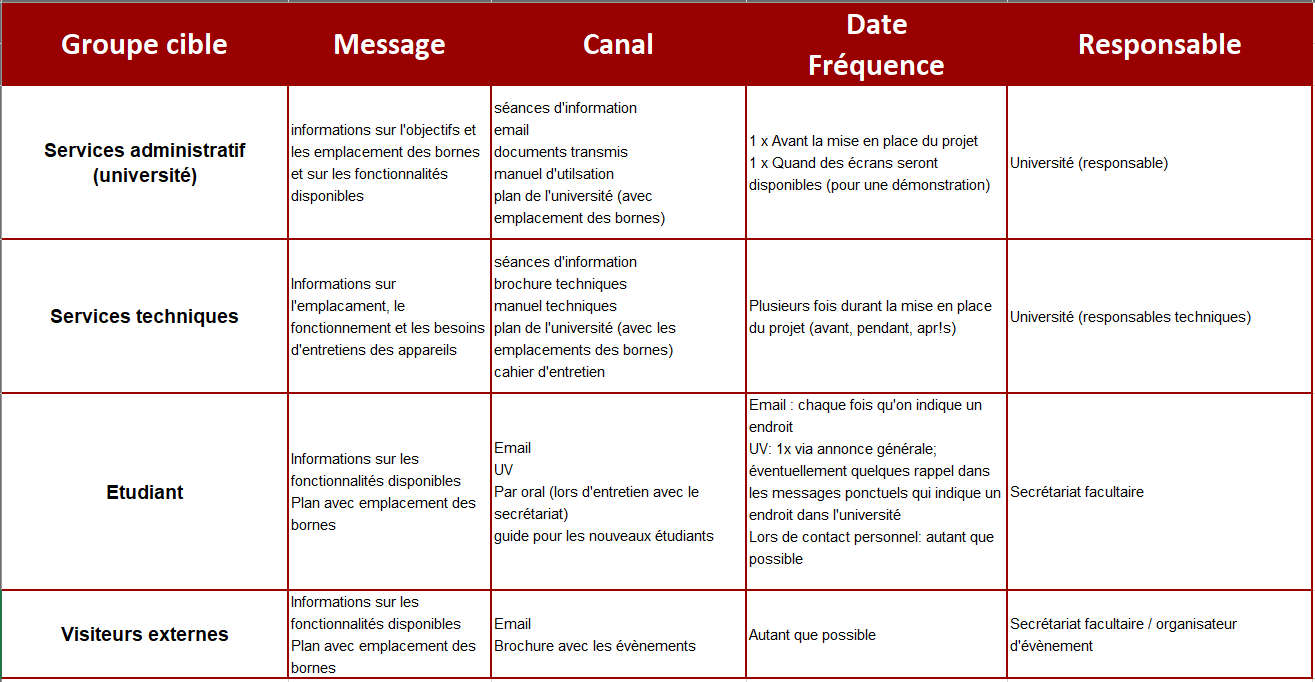
\includegraphics[width=16cm]{Pictures/tb_plan_com.png}
\caption{Plan de communication}
\label{plan_com}
\end{figure}